\documentclass{beamer}
\usepackage[latin1]{inputenc}
\usepackage{xcolor}
\usepackage{hyperref}
\usepackage{minted}
\usepackage{graphicx}
\usepackage{tikz}
\usetikzlibrary{shapes,fit,positioning,calc}

\usetheme{default}
\usecolortheme{default}

\title{COMP3320 Introduction to OpenGL}
\author{Alex Biddulph}
\institute{
    The University of Newcastle, Australia
    \and
    Based on the work provided at \url{www.learnopengl.com}
}
\date{Semester 2, 2019}

\begin{document}

\begin{frame}
\titlepage
\end{frame}

\begin{frame}[fragile]{The Open-Asset-Importer-Lib}
    \begin{itemize}
        \item Asset importer library supporting multiple 3D model formats
        \item Provides some post-processing support
        \item API provided for C/C++
        \item Languange bindings available for C\#, Java, Python, Delphi, D
        \item Can run on Android and iOS
        \item Check out \url{assimp.org}
    \end{itemize}
\end{frame}

\begin{frame}[fragile]{Assimp Importers}
    \begin{tabular}{cccc}
        3D & \textbf{3DS} & 3MF & AC \\
        AC3D & ACC & AMJ & ASE \\
        ASK & B3D & \textbf{BLEND} & BVH \\
        CMS & COB & \textbf{DAE/Collada} & DXF \\
        ENFF & FBX & glTF 1.0 + GLB & glTF 2.0 \\
        HMB & IFC-STEP & IRR / IRRMESH & LWO \\
        LWS & LXO & MD2 & MD3 \\
        MD5 & MDC & MDL & MESH / MESH.XML \\
        MOT & MS3D & NDO & NFF \\
        \textbf{OBJ} & OFF & OGEX & PLY \\
        PMX & PRJ & Q3O & Q3S \\
        RAW & SCN & SIB & SMD \\
        STP & \textbf{STL} & TER & UC \\
        VTA & X & X3D & XGL \\
            &   & ZGL &
    \end{tabular}
\end{frame}

\begin{frame}[fragile]{Assimp Post Processing Support}
    \begin{itemize}
        \item Normal generation
        \item Tangent generation
        \item Triangulation
        \item Removal of degenrate primitives
        \item Removal of duplicate vertices
        \item Index generation
        \item Lots more
    \end{itemize}
\end{frame}

\begin{frame}[fragile]{Assimp Model Structure}
    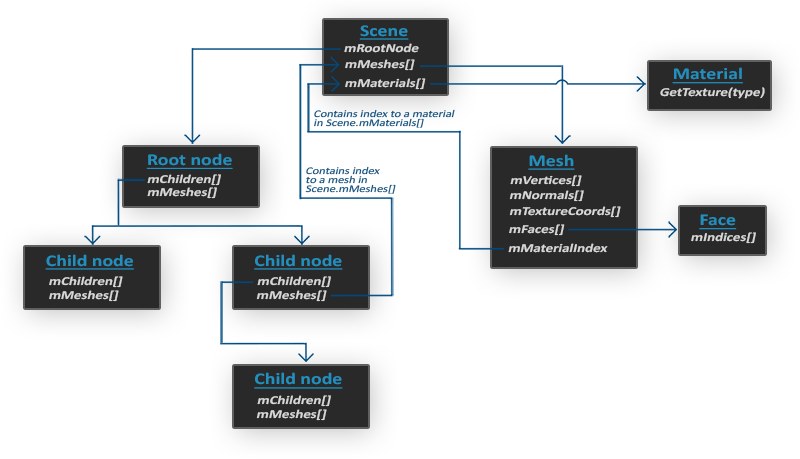
\includegraphics[width=\linewidth]{images/assimp_structure.png}
    {\footnotesize{Image sourced from \url{learnopengl.com/Model-Loading/Assimp}}}
\end{frame}

\begin{frame}[fragile]{Assimp Model Structure}
    \begin{itemize}
        \item {\color{blue}\verb"Scene"} is the root node of the imported model
        \item {\color{blue}\verb"Scene"} contains all meshes and materials as well as a link to root node of the meshes
        \item {\color{blue}\verb"Root Node"} starts a tree structure that contains links to meshes and child nodes
        \item Each {\color{blue}\verb"Mesh"} contains vertices, normals, texture coordinates, faces, and a link to
            materials (textures)
        \item Only vertices and faces is guaranteed to be in a {\color{blue}\verb"Mesh"}, the rest are only there if
            they were in the model or you asked Assimp to calculate them for you
        \item Each {\color{blue}\verb"Face"} contains indices
        \item Each {\color{blue}\verb"Material"} contains information about a texture
    \end{itemize}
\end{frame}

\begin{frame}[fragile]{Assimp and OpenGL}
    \begin{itemize}
        \item Not geared at OpenGL
        \item Best to restructure the {\color{blue}\verb"Scene"} data to make it easier to work with OpenGL
        \begin{itemize}
            \item Create our own {\color{blue}\verb"Vertex"} class which encapsulates position, normal, and texture
                coordinates
            \item Create our own {\color{blue}\verb"Mesh"} class which encapsulates VAOs, VBOs, EBOs,
                {\color{blue}\verb"Vertex"} data, and textures
            \item The {\color{blue}\verb"Mesh"} class can also bind its own textures and render its own indices/vertices
            \item The program's main render loop can now be reduced to calling {\color{blue}\verb"model.render()"} for
                each loaded model and setting up uniforms for lighting
        \end{itemize}
    \end{itemize}
\end{frame}

\begin{frame}[fragile]{OpenAL}
    \begin{itemize}
        \item Software interface for audio hardware
        \item Meant to resemble the OpenGL API
        \item A means to generate audio in a simulated 3D space
        \item OpenAL includes both the core API as well as OS bindings (unlike OpenGL)
        \item Can handle sound source directivity, distane-related attenuation, Doppler effects, and environmental
            effects
        \begin{itemize}
            \item Reflection,
            \item Obstruction,
            \item Transmission, and
            \item Reverberation
        \end{itemize}
    \end{itemize}
\end{frame}

\begin{frame}[fragile]{OpenAL Structure}
    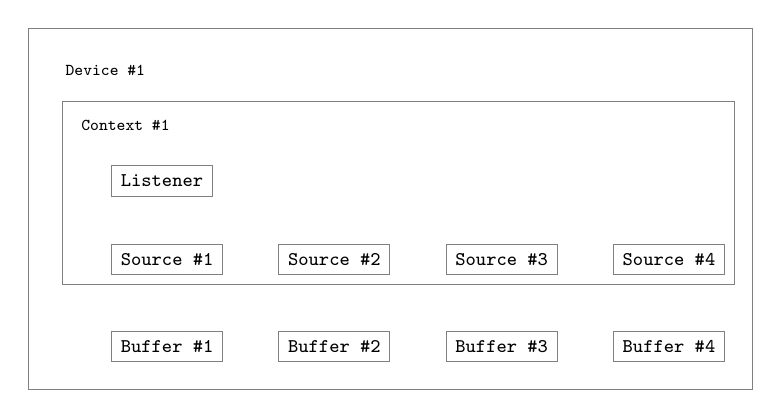
\begin{tikzpicture}[
        node distance=7mm,
        title/.style={font=\fontsize{6}{6}\color{black}\ttfamily},
        contexttag/.style={rectangle, draw=black!50, font=\scriptsize\ttfamily, anchor=west},
        devicetag/.style={rectangle, draw=black!50, font=\scriptsize\ttfamily}
    ]
        \node (device) [title] {Device \#1};

        \node (context) [below=of device.west, title, anchor=west, xshift=2mm] {Context \#1};

        \node (listener) [below=of context.west, contexttag, xshift=5mm] {Listener};
        \node (source1) [below=of context.west, contexttag, xshift=5mm, yshift=-1.0cm] {Source \#1};
        \node (source2) [right=of source1.east, contexttag] {Source \#2};
        \node (source3) [right=of source2.east, contexttag] {Source \#3};
        \node (source4) [right=of source3.east, contexttag] {Source \#4};

        \node [draw=black!50, fit={(context) (listener) (source1) (source2) (source3) (source4)}] {};

        \node (buffer1) [below=of source1.south, devicetag] {Buffer \#1};
        \node (buffer2) [right=of buffer1.east, devicetag] {Buffer \#2};
        \node (buffer3) [right=of buffer2.east, devicetag] {Buffer \#3};
        \node (buffer4) [right=of buffer3.east, devicetag] {Buffer \#4};

        \node [inner sep=10pt, draw=black!50, fit={(device) (context) (buffer1) (buffer2) (buffer3) (buffer4)}] {};
    \end{tikzpicture}
    \vfill{}
    {\footnotesize{Image recreated from \url{https://www.openal.org/documentation/OpenAL_Programmers_Guide.pdf}}}
\end{frame}

\begin{frame}[fragile]{OpenAL Structure}
    \begin{itemize}
        \item {\color{blue}\verb"Buffer"}s are filled with audio data
        \begin{itemize}
            \item Need to use an external library for this, similar to OpenGL and textures
            \item libsndfile is one option for this
        \end{itemize}
        \item A {\color{blue}\verb"Buffer"} is then attached to a {\color{blue}\verb"Source"}
        \item There can be multiple {\color{blue}\verb"Source"}s
        \item A {\color{blue}\verb"Source"} has a position and an orientation (and other properties)
        \item The position and orientation of a {\color{blue}\verb"Source"} relative to the {\color{blue}
            \verb"Listener"} dictates how the {\color{blue}\verb"Source"} is heard
        \item There can only be $1$ {\color{blue}\verb"Listener"}
        \item Update the positions and orientations of the {\color{blue}\verb"Listener"} and
            {\color{blue}\verb"Source"}s dynamically to get convincing 3D audio
    \end{itemize}
\end{frame}

\begin{frame}[fragile]{OpenAL Properties}
    \begin{itemize}
        \item {\color{blue}\verb"Listener"} properties
        \begin{itemize}
            \item Gain
            \item Position
            \item Velocity
            \item Orientation (\emph{position} $+$ \emph{up})
        \end{itemize}
        \item {\color{blue}\verb"Source"} properties
        \begin{itemize}
            \item Pitch
            \item Min gain, Gain, Max gain
            \item Max distance, Reference distance
            \item Rolloff factor
            \item Position, velocity, direction
            \item Source relative
            \item Looping
            \item .... many more
        \end{itemize}
    \end{itemize}
\end{frame}

\end{document}
